\section{Introduction to Dynamic Clamp}
\index{dynamic clamp}
Traditionally, the properties of electrically excitable cells are assessed using current clamp and voltage clamp electrophysiology protocols. In \textit{current clamp}, an electrical current waveform is specified and applied to the cell through a microelectrode while the transmembrane potential is recorded. In \textit{voltage clamp}, a desired voltage waveform is specified and analog circuitry is used to determine and inject a current that is necessary to maintain, or clamp, the membrane potential at the specified values. The \textit{dynamic clamp} allows the insertion of artificial membrane conductances, such as ion channels, by injecting current that is a function of the cell's membrane potential. The injected current is computed by computer software or analog circuitry based on the equivalent circuit model of an excitable cell (Fig. \ref{fig:circuit}). The artificial conductance is effectively in parallel with other membrane processes, each of which contributes to the total transmembrane current. 

\begin{figure} 
\begin{center}
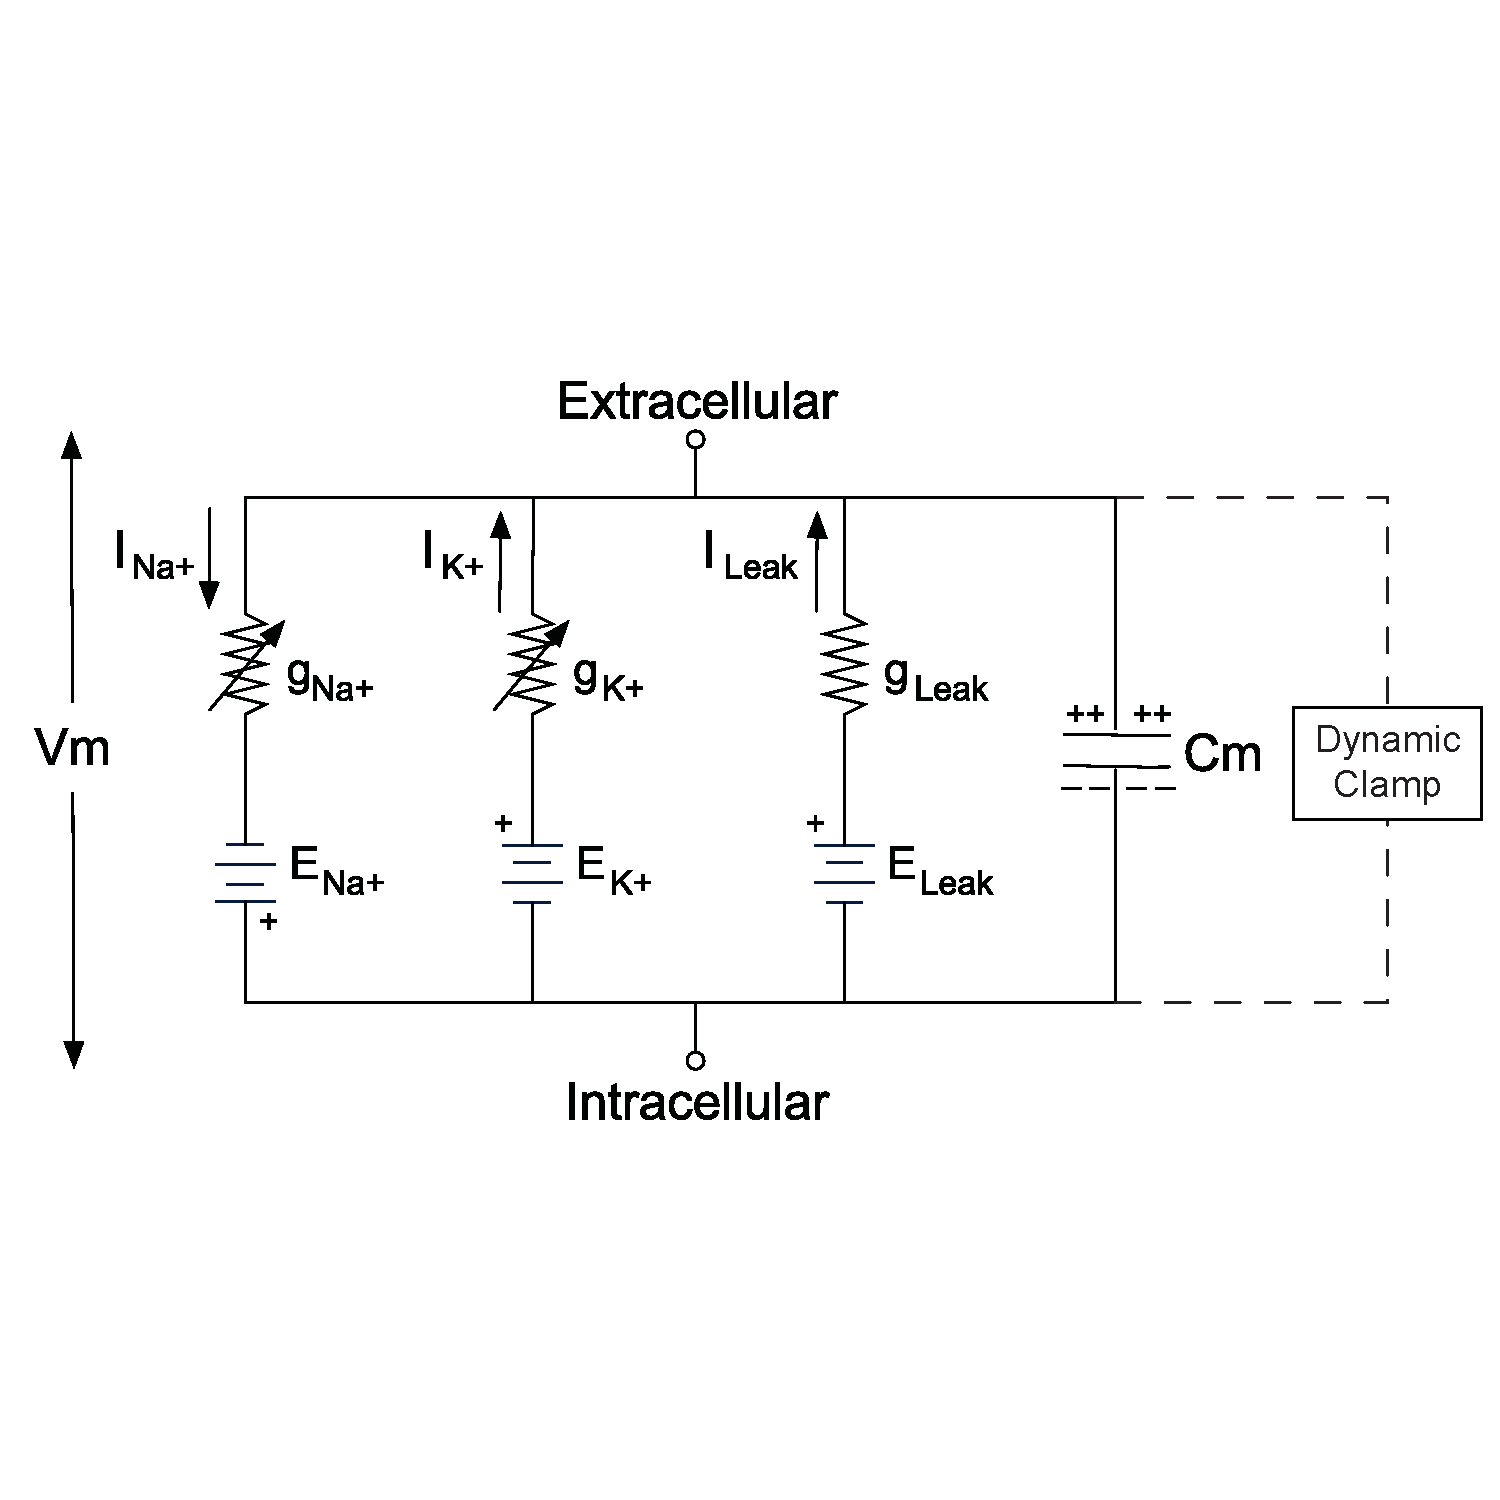
\includegraphics[width=4.5in]{dclampcircuit.pdf}
\caption[Equivalent circuit model of an excitable cell]{Equivalent circuit model of an excitable cell where $V_m$ represents the transmembrane potential, $C_m$ represents the membrane capacitance, and each conductance is defined by a reversal potential $E_{i}$ and a conductance $g_{i}$. In this model, the voltage-dependent sodium and potassium ion channels are depicted as variable resistors where $g_{i}=g_{i}(V_{m})$ . The reversal potential (or equilibrium potential) of an ion is the value of transmembrane voltage at which diffusive and electrical forces counterbalance, so that there is no net ion flow across the membrane. The reversal potential is represented as a battery since the potential difference $V_{\textrm{m}}-E_{i}$ gives the driving force across the membrane for that ionic current.} 
\label{fig:circuit} 
\end{center}
\end{figure}

The total transmembrane current is related to changes in the membrane potential, $V_{m}$, through the following equation: \index{neuron model}
\begin{eqnarray}
C_{m} \frac{dV_{m}}{dt} =-\Sigma I_{i}
\end{eqnarray}
where $C_{m}$ is the membrane capacitance. Any conductance that can be described mathematically can be applied to a neuron using the dynamic clamp. The current passing through an ion channel, for example, is often described by Ohm's law using the following conductance-based equation: 
\begin{eqnarray}\index{ion channel model}
I_{i} & = & g_{i}(V_{m})(V_{m}-E_{i}) \\
g_{i}(V_{m}) & = & \bar{g}_{i}m^{\textrm{p}}h^{\textrm{q}} 
\end{eqnarray}
where $\bar{g}$ is the maximal conductance, and $m$ and $h$ are voltage-dependent activation and inactivation gating variables ($p$ and $q$ are integers) that describe the kinetic activation of the channel. Gating variables have values between 0 and 1 to scale the channel conductance and are typically described by a first order differential equation:
\begin{eqnarray}
\frac{dx}{dt} & = & \frac{x_{\infty}(V_{m})-x}{\tau (V_{m})} 
\end{eqnarray}
The membrane potential is re-sampled and the equations are re-evaluated on every computational cycle of the dynamic clamp system. As such, the dynamic clamp is also sometimes termed \textit{conductance clamp} or \textit{conductance injection}. 

While the dynamic clamp was first demonstrated in cardiac electrophysiology to electrically couple embryonic chick myocytes \cite{Wilders:2006p930}, the technique was independently introduced \cite{Robinson:1993p1193,Sharp:1993p983} and is now more prevalent in neural electrophysiology \cite{Economo:2010p1795,Prinz:2004p985,Goaillard:2006p1175}. Applications of this technique include the insertion of non-native ion channels (a virtual ``knock-in''), subtraction of native ion channels (a virtual ``knock-out"), and simulation of synapses and electrical gap junctions to create small networks of biological and/or simulated neurons. By varying the parameter values of a model channel or synapse, experiments can be conducted to determine how these properties shape membrane dynamics and neuron activity. These approaches have made the dynamic clamp a valuable tool for studying the intrinsic properties of single neurons and the behavior of small neural networks. 

Dynamic clamp studies have also made important contributions to our understanding of neuronal dynamics under in vivo-like conditions in which neurons receive a constant barrage of synaptic inputs which can easily reach thousands of events per second. Artificial synaptic input can be constructed from pre-recorded activity of presynaptic neurons but is more commonly based on statistical descriptions of noisy conductance waveforms. This high conductance state has been shown to enhance the cell's responsiveness to small inputs, also known as its gain \cite{Chance:2002p1075,Destexhe:2003p1021,Sceniak:2010p1258}, and can change the signal integration of synaptic input, creating distinct modes of firing patterns \cite{Wolfart:2005p1138,Steriade:2001p4667,Rudolph:2003p4555,Destexhe:2001p1044}. The statistics of current-based versus conductance-based input, such as correlations and relative balance between excitation and inhibition, are translated differently into output statistics such as the membrane potential distribution, the distribution of interspike intervals (ISIs), the coefficient of variation (CV), and the mean and variance of the neuron's output firing rate \cite{Tiesinga:2000p1134,Rudolph:2003p4554,Kumar:2008p4586,Salinas:2000p4826}. Together, these factors result in a dynamical behavior of the neuron that is usually quite different from the intrinsic dynamics of the voltage-gated currents. 

Results from dynamic clamp experiments must be carefully interpreted due to several experimental limitations. Space-clamp problems arise in that the injected current is limited to a space around the recording electrode. In some experimental studies, an artificial dendrite is modeled as well to simulate the cable effects of synaptic inputs propagating to the action potential initiation zone \cite{Hughes:2008p993}. Since current can usually only be injected at the soma, the dynamic clamp may be a poor approximation of dendritic input in some cell types. In most cells, the dynamic clamp is operated in discontinuous current clamp (DCC) mode in which a single electrode switches between recording and current injection states. In this configuration, it is not possible to inject large conductances that approach the magnitude of the cell's intrinsic resting conductance while still accurately recording the membrane potential. The injected current induces a voltage drop through the electrode and causes measurement accuracies that are propagated through the closed feedback loop in the dynamic clamp system and may cause ringing artifacts in the recording \cite{Brizzi:2004p935,Jaeger:1999p1094,Preyer:2007p359,Preyer:2009p1228}. In larger cells, two electrodes may be used, one to record and one to inject current. Researchers also typically use the same ion channel or synapse model parameters for all cells used in an experiment, assuming that neurons of the same cell type have identical intrinsic properties, both within an animal and between animals \cite{Golowasch:2002p5763}. There usually is not time during an experiment to manually adjust the model to optimal parameters for each cell.

Compared to other real-time closed-loop experimental protocols, the dynamic clamp has perhaps the most stringent performance requirements. These limitations involve numerical, algorithmic, and hardware platform-specific issues. Dynamic clamp performance depends on how accurately the model is solved, measurement error in sampling the voltage, and the sampling rate of the system. \index{sampling rate}The sampling rate determines how much time is in a given computational cycle for various operations to be performed, and the duration of the cycle restricts the types of numerical methods that may be used to integrate the gating variables. Thus, the computational performance of dynamic clamp suffers from a trade-off between the speed of computation and numerical accuracy. Dynamic clamp sampling rates are currently chosen based on the limits of the hardware platform being used and the temporal dynamics being simulated. While it is possible to compute the time step necessary for the Euler and exponential Euler methods to achieve a desired one-step integration accuracy for a known voltage measurement error, few studies employ this technique \cite{Butera:2004p1073}. In simulations of dynamic clamp, Euler integration was insufficient to model fast sodium Na$_{v}$ channels at sampling rates under 30 kHz and nearly identical integration results for three different deterministic integration methods was only achieved at rates $\geq$50 kHz \cite{Milescu:2008p1216}. Standard performance benchmarks are needed for dynamic clamp to justify the sampling rates that are used.

Other hardware that are typically required for dynamic clamp are an electrophysiology amplifier for measuring membrane potential and injecting current and a multifunctional data acquisition system (DAQ) for performing analog-to-digital (ADC) and digital-to-analog (DAC) conversion. The technical specifications of each of these hardware components can affect the performance of the overall system by introducing additional jitter, latency, and quantization error that can affect system timing and the numerical computation \cite{Bettencourt:2008p1114, Butera:2001p910}. Recent results show that faster systems would result in a greater range of conductances that could be utilized, improved stability, and more accurate real-time model simulations \cite{Preyer:2007p359,Preyer:2009p1228}. Faster dynamic clamp systems have been developed, largely due to the increasing power of personal computers, but also due to the development of systems based on the GNU/Linux operating system and embedded real-time processors. 